\section{Événements simulés}\label{chapter-LHC-section-MC}
La simulation d'événements permet de comparer les résultats expérimentaux aux prédictions théoriques.
Elle se déroule en deux temps.
\par Premièrement, les processus physiques prédits par le modèle théorique à tester sont simulés.
La nature probabiliste des ces processus mène à utiliser un générateur d'événements Monte-Carlo.
Cette étape est détaillée en section~\ref{chapter-LHC-section-MC-subsec-evt_gen}.
Les particules issues des collisions sont alors obtenues ainsi que toute l'historique de leurs formations à partir des particules initiales entrant en collision.
\par Deuxièmement, la propagation de ces particules dans le détecteur, leurs interactions avec ses différents composants et les signaux qui en résultent sont également simulés.
Cette simulation du détecteur est l'objet de la section~\ref{chapter-LHC-section-MC-subsec-detector_sim}.
Cette méthode permet d'obtenir une estimation des signaux devant être observés avec le détecteur si le modèle testé est le modèle décrivant effectivement l'Univers.
\subsection{Génération d'événements}\label{chapter-LHC-section-MC-subsec-evt_gen}
Lorsque deux protons entrent en collision, ce sont leurs constituants respectifs interagissent.
Ces constituants portent une fraction $x$ de l'énergie totale du proton, comme expliqué dans la section~\ref{chapter-LHC-section-LHC-subsec-pp_collisions}.
Le nombre de constituants différents en jeu ainsi que leurs modes d'interactions peuvent donner une structure de l'événement complexe, comme illustré sur la figure~\ref{fig-event_generator_HEP-2-Figure1-1}.
\begin{figure}[h]
\centering
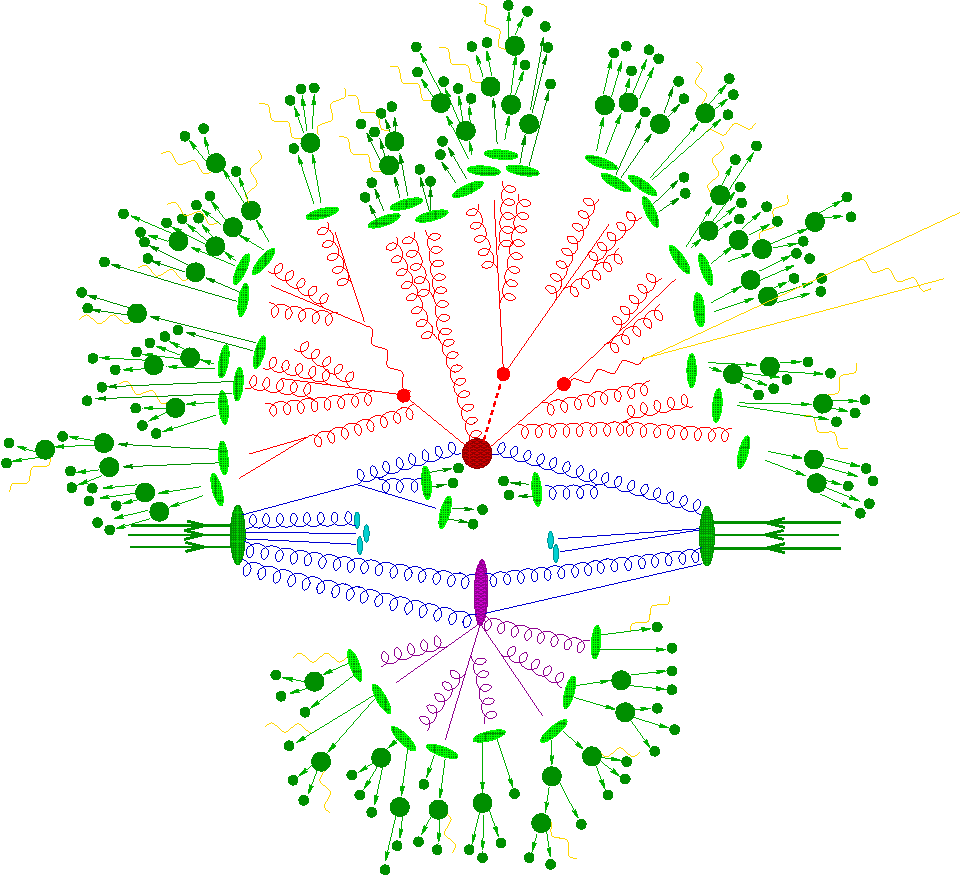
\includegraphics[width=15cm]{\PhDthesisdir/plots_and_images/from_event_generator_HEP/2-Figure1-1.tex}
\caption[Représentation d'une collision de protons.]{Représentation d'une collision de protons~\cite{event_generator_HEP}.}
\label{fig-event_generator_HEP-2-Figure1-1}
\end{figure}
\par La description analytique des ces événements est réalisée grâce à la théorie des perturbations.
À l'aide des règles de Feynman présentées dans l'annexe~\refApFmf, il est possible de calculer l'\og élément de matrice \fg{} permettant de décrire le passage d'un état initial à un état final.
Les événements sont alors générés à un ordre perturbatif donné.
La plupart des processus sont ainsi disponibles à l'ordre dominant (LO, \emph{Leading Order}).
Leur génération peut se faire par des générateurs~\cite{CAVENDISH-HEP-10-21}, comme
\MADGRAPH~\cite{madgraph5} et
\PYTHIA~\cite{pythia6.4,pythia8.2}.
Dans certains cas, les ordres supérieurs (NLO, \emph{Next-to-Leading Order}, NNLO, \emph{Next-to-Next-to-Leading Order}, etc.) sont également disponibles grâce à des générateurs NLO tels que
\POWHEG~\cite{Alioli:2010xd} et
\MCATNLO~\cite{MCATNLO}.
\par Ces générateurs donnent ainsi le processus initial de la collision, duquel sont issues de nouvelles particules.
Cependant, les particules possédant une charge de couleur comme les quarks ne peuvent subsister seules à cause du confinement de couleur, phénomène abordé dans le chapitre~\refChMSSM.
Des étapes de génération supplémentaires sont alors nécessaires afin de décrire l'évolution ultérieure de ces particules.
Il s'agit de la formation de la gerbe partonique et de l'hadronisation, détaillées dans le chapitre~\refChHLO.
Des générateurs comme
\PYTHIA~\cite{pythia6.4,pythia8.2} et
\HERWIG~\cite{herwig}
permettent de simuler le processus initial ainsi que ces étapes ultérieures.
\par Enfin, lors d'une collision de protons et plus généralement de hadrons, plusieurs interactions entre les constituants des hadrons peuvent survenir.
L'interaction emportant la plus grande fraction de l'énergie des hadrons est l'\og interaction dure \fg{}.
Les autres interactions constituent l'événement sous-jacent.
\subsection{Simulation du détecteur}\label{chapter-LHC-section-MC-subsec-detector_sim}
Une fois simulée la physique de l'événement, indépendante du détecteur utilisé, il faut simuler la réponse du détecteur à cet événement.
La propagation des particules est alors simulée en prenant en compte la présence du champ magnétique courbant les trajectoires des particules chargées.
\par Les désintégrations de certaines particules ont lieu dans le volume du détecteur et sont également simulées.
La modélisation du détecteur permet de simuler les déviations des particules dues à la traversée de la matière constituant le détecteur~\cite{moliere_scat_1,moliere_scat_2} ainsi que les interactions propres à la détection de ces particules comme les traces, les gerbes électromagnétiques et hadroniques.
Alors, la modélisation de l'électronique et du système de déclenchement donnent une simulation de la réponse complète du détecteur à l'événement physique généré.
\par Cette simulation du détecteur est basée sur le logiciel
\GEANTfour~\cite{geant4_2003,geant4_2006,geant4_2016}.
La modélisation du câblage interne du détecteur permet d'obtenir des résultats fidèles à la réalité.
Les signaux simulés du détecteur ainsi obtenus sont alors traités, comme dans le cas des données réelles, par l'algorithme de \emph{Particle Flow}, abordé dans la section suivante, permettant de reconstruire l'événement physique à partir des signaux du détecteur.